\begin{pastexam}[label={px:gk3-107-ds-03}]{高考三級資訊處理 107 年 第三題}
（申論；20 分）

一無向圖 G 之節點集合為 G(V)=\{0,1,2,3,4,5,6,7,8,9\}，邊集合為 G(E)=\{(0,1), (1,2), (1,3), (2,4), (3,4), (3,5),
(5,6), (5,7), (6,7), (7,8), (7,9)\}；請列出 G 之接合點（articulation point）和畫出 G 的所有雙連通元件（biconnected
component），雙連通元件須以節點和邊構成之子圖方式表示。（20 分）
\end{pastexam}

\begin{pastsoln}
答案：接合點是 $1, 3, 5, 7$。 雙連通元件共 $6$ 個：$\{0, 1\}$；$\{1, 2, 3, 4\}$（四條邊的環）；$\{3, 5\}$；
$\{5, 6, 7\}$（三角形）；$\{7, 8\}$；$\{7, 9\}$。

先把圖畫出來：
\begin{center}
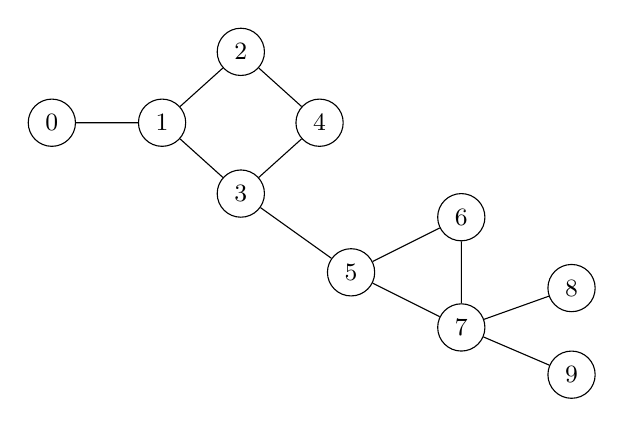
\begin{tikzpicture}[v/.style={circle,draw,minimum size=6mm,inner sep=0pt,font=\small}]
\node[v] (0) at (0,0) {0};
\node[v] (1) at (1.4,0) {1};
\node[v] (2) at (2.4,0.9) {2};
\node[v] (3) at (2.4,-0.9) {3};
\node[v] (4) at (3.4,0) {4};
\node[v] (5) at (3.8,-1.9) {5};
\node[v] (6) at (5.2,-1.2) {6};
\node[v] (7) at (5.2,-2.6) {7};
\node[v] (8) at (6.6,-2.1) {8};
\node[v] (9) at (6.6,-3.2) {9};
\draw (0)--(1) (1)--(2) (1)--(3) (2)--(4) (3)--(4) (3)--(5) (5)--(6) (5)--(7) (6)--(7) (7)--(8) (7)--(9);
\end{tikzpicture}
\end{center}

\textbf{用 DFS 求接合點}（資結書第~23.5~節）。 從 $0$ 出發，相鄰頂點依編號由小到大走。 $\mathit{dfn}[u]$ 是
$u$ 被拜訪的順序，$\mathit{low}[u]$ 是從 $u$ 的子樹出發、走樹邊往下再走最多一條回邊，能到達的最小
$\mathit{dfn}$。 DFS 的走法：$0 \to 1 \to 2 \to 4 \to 3 \to 5 \to 6 \to 7 \to 8$，回到 $7$ 再走 $9$。 回邊有兩條：
$(3, 1)$ 和 $(7, 5)$。
\begin{center}
\small
\begin{tabular}{l*{10}{c}}
\toprule
頂點 $u$ & 0 & 1 & 2 & 4 & 3 & 5 & 6 & 7 & 8 & 9 \\
\midrule
$\mathit{dfn}[u]$ & 1 & 2 & 3 & 4 & 5 & 6 & 7 & 8 & 9 & 10 \\
$\mathit{low}[u]$ & 1 & 2 & 2 & 2 & 2 & 6 & 6 & 6 & 9 & 10 \\
\bottomrule
\end{tabular}
\end{center}
（$3$ 有回邊到 $1$，所以 $\mathit{low}[3] = 2$，再往上傳給 $4$、$2$；$7$ 有回邊到 $5$，$\mathit{low}[7] = 6$，
傳給 $6$。）

判斷規則（資結書定理~23.8、23.9）：根是接合點若且唯若它在 DFS 樹中有兩個以上子節點；非根 $u$ 是接合點若且
唯若它有某個子節點 $w$ 滿足 $\mathit{low}[w] \ge \mathit{dfn}[u]$。
\begin{itemize}
\item 根 $0$ 只有一個子節點 $1$：不是。
\item $1$：子節點 $2$ 的 $\mathit{low} = 2 \ge \mathit{dfn}[1] = 2$，\textbf{是}（拿掉 $1$，$0$ 就孤立）。
\item $2$：子節點 $4$ 的 $\mathit{low} = 2 < 3$；$4$：子節點 $3$ 的 $\mathit{low} = 2 < 4$。 都不是。
\item $3$：子節點 $5$ 的 $\mathit{low} = 6 \ge 5$，\textbf{是}。
\item $5$：子節點 $6$ 的 $\mathit{low} = 6 \ge 6$，\textbf{是}。
\item $6$：子節點 $7$ 的 $\mathit{low} = 6 < 7$，不是。
\item $7$：子節點 $8$ 的 $\mathit{low} = 9 \ge 8$（$9$ 也一樣），\textbf{是}。
\item $8$、$9$ 是葉子，不是。
\end{itemize}
接合點：$\mathbf{1, 3, 5, 7}$。

\textbf{雙連通元件}：極大的、沒有接合點的連通子圖；每條邊恰好屬於一個元件，接合點會出現在好幾個元件裡
（資結書第~23.6~節）。 DFS 時把邊推進堆疊，每遇到 $\mathit{low}[w] \ge \mathit{dfn}[u]$ 就把堆疊彈到邊 $(u, w)$
為止，彈出的邊就是一個元件。 依彈出順序：
\begin{center}
\small
\begin{tabular}{cll}
\toprule
元件 & 頂點 & 邊 \\
\midrule
$B_1$ & $\{7, 8\}$ & $(7,8)$ \\
$B_2$ & $\{7, 9\}$ & $(7,9)$ \\
$B_3$ & $\{5, 6, 7\}$ & $(5,6), (6,7), (5,7)$ \\
$B_4$ & $\{3, 5\}$ & $(3,5)$ \\
$B_5$ & $\{1, 2, 3, 4\}$ & $(1,2), (2,4), (3,4), (1,3)$ \\
$B_6$ & $\{0, 1\}$ & $(0,1)$ \\
\bottomrule
\end{tabular}
\end{center}
十一條邊都恰好出現一次。 子圖如下（接合點加粗）：
\begin{center}
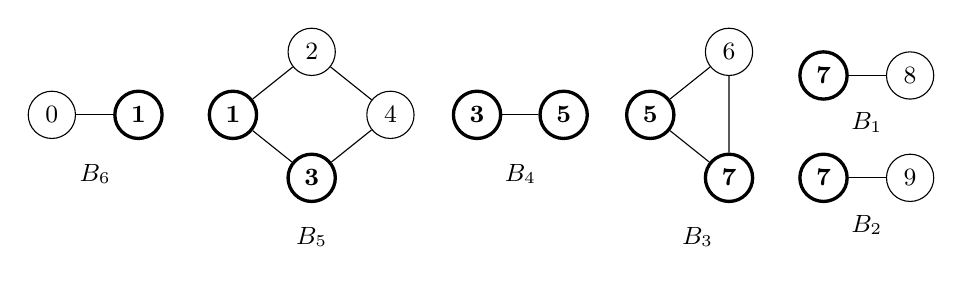
\begin{tikzpicture}[v/.style={circle,draw,minimum size=6mm,inner sep=0pt,font=\small},
  a/.style={circle,draw,very thick,minimum size=6mm,inner sep=0pt,font=\small\bfseries}]
\node[v] (a0) at (0,0) {0}; \node[a] (a1) at (1.1,0) {1};
\node at (0.55,-0.75) {\small $B_6$};
\begin{scope}[xshift=2.3cm]
\node[a] (b1) at (0,0) {1}; \node[v] (b2) at (1,0.8) {2}; \node[a] (b3) at (1,-0.8) {3}; \node[v] (b4) at (2,0) {4};
\draw (b1)--(b2)--(b4)--(b3)--(b1);
\node at (1,-1.55) {\small $B_5$};
\end{scope}
\begin{scope}[xshift=5.4cm]
\node[a] (c3) at (0,0) {3}; \node[a] (c5) at (1.1,0) {5};
\draw (c3)--(c5);
\node at (0.55,-0.75) {\small $B_4$};
\end{scope}
\begin{scope}[xshift=7.6cm]
\node[a] (d5) at (0,0) {5}; \node[v] (d6) at (1,0.8) {6}; \node[a] (d7) at (1,-0.8) {7};
\draw (d5)--(d6)--(d7)--(d5);
\node at (0.6,-1.55) {\small $B_3$};
\end{scope}
\begin{scope}[xshift=9.8cm]
\node[a] (e7) at (0,0.5) {7}; \node[v] (e8) at (1.1,0.5) {8};
\draw (e7)--(e8);
\node at (0.55,-0.1) {\small $B_1$};
\node[a] (f7) at (0,-0.8) {7}; \node[v] (f9) at (1.1,-0.8) {9};
\draw (f7)--(f9);
\node at (0.55,-1.4) {\small $B_2$};
\end{scope}
\draw (a0)--(a1);
\end{tikzpicture}
\end{center}
檢查：$\{1,2,3,4\}$ 是一個環、$\{5,6,7\}$ 是三角形，拿掉任一點都還連通；其餘四個元件各是一條邊（橋），單一
條邊也是雙連通元件。 接合點 $1$ 在 $B_5, B_6$，$3$ 在 $B_4, B_5$，$5$ 在 $B_3, B_4$，$7$ 在 $B_1, B_2, B_3$。
\end{pastsoln}
